\documentclass[12pt]{article}

\usepackage{amsmath,amssymb,amsfonts,amsthm}
\usepackage{array,booktabs,longtable,multirow}
\usepackage{graphicx,float}
\usepackage{tikz}
\usetikzlibrary{arrows.meta,positioning,fit,patterns}
\usepackage[colorlinks=true,linkcolor=blue,citecolor=blue,urlcolor=blue]{hyperref}
\usepackage[margin=2.7cm]{geometry}

\parskip=3pt
\setlength{\parindent}{15pt}
\setlength{\abovedisplayskip}{6pt plus 2pt minus 2pt}
\setlength{\belowdisplayskip}{6pt plus 2pt minus 2pt}
\setlength{\abovedisplayshortskip}{3pt plus 1pt minus 1pt}
\setlength{\belowdisplayshortskip}{4pt plus 1pt minus 1pt}
\allowdisplaybreaks

\newtheorem{thm}{Theorem}[section]
\newtheorem{lem}[thm]{Lemma}
\newtheorem{prop}[thm]{Proposition}
\newtheorem{coro}[thm]{Corollary}
\newtheorem{deff}[thm]{Definition}
\newtheorem{exa}[thm]{Example}
\newtheorem{remark}[thm]{Remark}

\newcommand{\cL}{\mathcal L}
\newcommand{\Comp}{\mathcal C}
\newcommand{\pattern}[4]{%
  \raisebox{0.6ex}{%
    \begin{tikzpicture}[scale=0.35,baseline=(current bounding box.center),#1]
      \if\relax\detokenize{#4}\relax\else
        \foreach \x/\y in {#4} \fill[gray!50] (\x,\y) rectangle +(1,1);
      \fi
      \draw (0.01,0.01) grid (#2+0.99,#2+0.99);
      \foreach \x/\y in {#3} \filldraw (\x,\y) circle (5.5pt);
    \end{tikzpicture}}
}

\newcommand{\activepattern}[5]{%
  \raisebox{0.6ex}{%
    \begin{tikzpicture}[scale=0.46,baseline=(current bounding box.center),#1]
      \foreach \x/\y in {#4} {
        \fill[blue!10] (\x,\y) rectangle +(1,1);
        \fill[pattern=north east lines,pattern color=blue!70!black]
          (\x,\y) rectangle +(1,1);
      }
      \foreach \x/\y in {#5} {
        \fill[orange!18] (\x,\y) rectangle +(1,1);
        \fill[pattern=dots,pattern color=orange!80!black]
          (\x,\y) rectangle +(1,1);
      }
      \draw[line width=0.35pt] (0.01,0.01) grid (#2+0.99,#2+0.99);
      \foreach \x/\y in {#3} \filldraw (\x,\y) circle (5.5pt);
    \end{tikzpicture}}
}

\begin{document}

\begin{center}
{\large The complete equidistribution classification of\\
length-three mesh patterns on layered permutations}
\end{center}

\begin{center}
{\large Jiahao Zhang}\\[10pt]
College of Mathematical Sciences \& Institute of Mathematics and
Interdisciplinary Sciences\\
Tianjin Normal University\\
Tianjin 300387, P. R. China
\end{center}

\noindent\textbf{Abstract.}
Distributional results for short mesh patterns have largely concerned selected
pattern families and host classes.  On layered permutations, length-two mesh
patterns form $35$ distribution classes, whereas at length three there are
$6\cdot2^{16}=393{,}216$ mesh patterns.  Here we classify all length-three
mesh patterns on the same host class.  For patterns whose underlying
permutation is
layered, we introduce a layer-constraint signature and derive occurrence and
signature-enumeration formulas valid at arbitrary length.  At length three,
the signature reduction, pointwise identities, composition bijections, and
two nonlocal identities yield exactly $146$ nonzero distribution classes.
The two non-layered underlying permutations contribute a single zero class,
giving $147$ classes in total.  Each equidistribution used for the upper bound
is proved for hosts of every size, and pairwise separation of the $146$
representatives gives the matching lower bound.

\par\smallskip\noindent\textbf{Keywords:} mesh pattern, layered permutation,
equidistribution, composition, classification.

\par\smallskip\noindent\textbf{2020 Mathematics Subject Classification:}
05A05, 05A15.

\section{Introduction}

Let $S_n$ denote the set of permutations of $[n]=\{1,\ldots,n\}$.  If
$\pi=\pi_1\cdots\pi_n\in S_n$ and $\tau=\tau_1\cdots\tau_k\in S_k$, an
\emph{occurrence} of the classical pattern $\tau$ in $\pi$ is a sequence of
indices $1\le i_1<\cdots<i_k\le n$ such that
\[
\pi_{i_a}<\pi_{i_b}
\quad\Longleftrightarrow\quad
\tau_a<\tau_b
\qquad(1\le a,b\le k).
\]
Thus the selected entries have the same relative order as $\tau$.  For
example, the subsequence $\pi_1\pi_2\pi_4=254$ of $\pi=25143$ is an occurrence
of $132$.  We refer to Kitaev~\cite{KitaevBook} for general background on
classical permutation patterns.

Mesh patterns, introduced by Br\"and\'en and Claesson~\cite{BrCl}, refine this
notion by imposing emptiness conditions around a classical occurrence.  A
mesh pattern of length $k$ is a pair $p=(\tau,R)$, where $\tau\in S_k$ and
$R\subseteq[0,k]\times[0,k]$, with $[0,k]=\{0,1,\ldots,k\}$.  Fix an occurrence at positions
$i_1<\cdots<i_k$, let $v_1<\cdots<v_k$ be its selected values in increasing
order, and set
\[
i_0=v_0=0,
\qquad
i_{k+1}=v_{k+1}=n+1.
\]
It is an occurrence of $p$ when, for every $(a,b)\in R$, the open rectangle
$(i_a,i_{a+1})\times(v_b,v_{b+1})$ contains no point $(j,\pi_j)$.  In the
standard diagram one plots the points $(a,\tau_a)$ and shades the unit cells
indexed by $R$.  For example,
\begin{center}
\pattern{scale=0.55}{3}{1/1,2/3,3/2}{0/0,1/1,1/2,3/1}
\qquad
$p=\bigl(132,\{(0,0),(1,1),(1,2),(3,1)\}\bigr)$.
\end{center}
The entries $243$ in the permutation $1243$ form a classical occurrence of
$132$, but not an occurrence of the displayed mesh pattern: the unselected
point $(1,1)$ lies in the shaded cell $(0,0)$.  By contrast, the first three
entries of $1324$ do form an occurrence, since its only unselected point lies
in the unshaded cell $(3,3)$.  To save space, throughout the paper we write
the underlying permutation in one-line notation and record the shaded set
algebraically; after the layer reduction we use the still more compact
signature notation.

Write $p(\pi)$ for the number of occurrences of $p$ in $\pi$.  For a fixed
host family $\mathcal C$, define
\[
D^{\mathcal C}_{p,n}(q)
=
\sum_{\substack{\pi\in\mathcal C\\|\pi|=n}}q^{p(\pi)}.
\]
Two patterns are \emph{distribution equivalent} on $\mathcal C$ when these
polynomials agree for every $n$.  This is distinct from coincidence, which
asks for equality of the avoidance sets, and from Wilf-equivalence, which
asks only for equality of their cardinalities.  Because a mesh pattern of
length $k$ has $(k+1)^2$ cells, there are
$k!\,2^{(k+1)^2}$ raw patterns.  Our problem is to classify the
$6\cdot2^{16}=393{,}216$ patterns of length three by distribution equivalence
when $\mathcal C$ is the class of layered permutations.

The literature on short mesh patterns began with avoidance.  Hilmarsson
\emph{et al.}~\cite{Hilmarsson} initiated the Wilf-classification at length
two, reducing the $1{,}024$ raw patterns to at most $65$ candidates and then to
an upper bound of $56$ Wilf-classes.  Kitaev and Zhang~\cite{KZ2019} began the
systematic study of full occurrence distributions for these patterns.
Further length-two equidistributions and infinite-family extensions were
obtained by Han and Zeng~\cite{HanZeng2021} and by Kitaev, Zhang, and
Zhang~\cite{KZZ2020}.  Related short-pattern statistics have also been pursued on restricted
hosts, including alternating
permutations~\cite{KitaevRemmel2013,HanKitaevZhang2025}, while distributions
of selected ordinary length-two mesh patterns have been studied on king
permutations~\cite{LiZhang2026}.

At length three, Bean, Gudmundsson, Magnusson, and
Ulfarsson~\cite{BeanEtAl2023} completed the coincidence classification.  That
result determines when two patterns have exactly the same avoiders, but it
does not determine their full occurrence distributions.  Distributional work
at length three has instead concentrated on structured subfamilies, notably
joint equidistributions of mesh patterns with underlying permutations $123$
and $132$ or $123$ and $321$ and with symmetric or minus-antipodal shadings
\cite{LvKitaev2025,LvZhang123132,LvZhang123321}.  Thus, despite substantial
progress, these studies do not classify the distributions of all
$393{,}216$ length-three mesh patterns.

Layered permutations provide a setting in which a complete result becomes
possible.  They form a natural and well-studied permutation class
\cite{AEPV}; every layered permutation is encoded by a composition, and every
classical occurrence has a canonical description in terms of supporting
layers.  Our recent length-two classification on this class
\cite{ZKPSlengthtwo} used that description case by case and obtained $35$
distribution classes.  To the best of our knowledge, the present paper is the
first to show that the full distributional classification of length-three mesh
patterns can also be completed on a specified nontrivial host class.

The layer-constraint signature is the main organizing device.  The active-cell
theorem and the signature formula are valid for mesh patterns of arbitrary
length whose underlying permutation is layered.  They yield a rational
generating function for total occurrences and an explicit enumeration of
signatures.  At length three, these tools reduce the $393{,}216$ raw diagrams
to $1{,}600$ effective shadings and then to $644$ signatures.  Pointwise
identities, reverse-complement, the unique-support classification,
layer-coordinate relabellings, and five families of distributional bridges
then give $146$ nonzero distribution classes.  The two non-layered underlying
permutations contribute one zero class.  Figure~\ref{fig:classification-flow}
records the intermediate quotients, and
Theorem~\ref{thm:146} establishes the matching upper and lower bounds.

\begin{figure}[htbp]
\centering
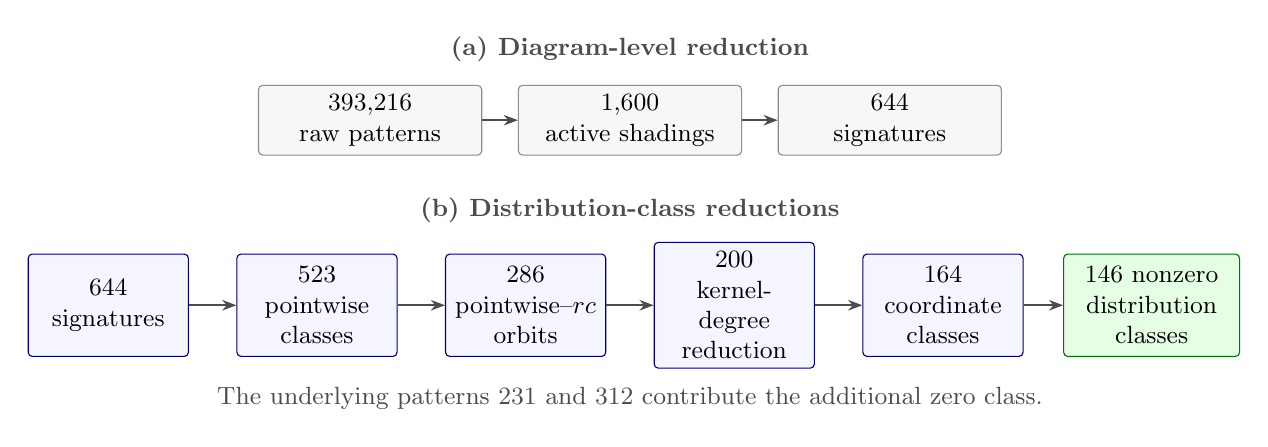
\begin{tikzpicture}[
  prebox/.style={draw=black!45,rounded corners=1.5pt,align=center,
                 minimum height=7.5mm,text width=2.6cm,fill=black!3,
                 font=\small},
  stage/.style={draw=blue!45!black,rounded corners=1.5pt,align=center,
                minimum height=13mm,text width=1.80cm,fill=blue!4,
                font=\small},
  finalstage/.style={stage,draw=green!45!black,fill=green!10},
  arr/.style={-{Stealth[length=1.8mm]},semithick,draw=black!70}
]
\node[font=\small\bfseries,text=black!70] at (0,3.25)
  {(a) Diagram-level reduction};
\node[prebox] (raw) at (-3.3,2.35) {$393{,}216$\\raw patterns};
\node[prebox] (active) at (0,2.35) {$1{,}600$\\active shadings};
\node[prebox] (presig) at (3.3,2.35) {$644$\\signatures};
\draw[arr] (raw)--(active);
\draw[arr] (active)--(presig);

\node[font=\small\bfseries,text=black!70] at (0,1.20)
  {(b) Distribution-class reductions};
\node[stage] (sig) at (-6.625,0.00) {$644$\\signatures};
\node[stage] (point) at (-3.975,0.00) {$523$\\pointwise\\classes};
\node[stage] (rc) at (-1.325,0.00) {$286$\\pointwise--$rc$\\orbits};
\node[stage] (kernel) at (1.325,0.00) {$200$\\kernel-degree\\reduction};
\node[stage] (layer) at (3.975,0.00) {$164$\\coordinate\\classes};
\node[finalstage,text width=2.00cm] (dist) at (6.625,0.00)
  {$146$ nonzero\\distribution\\classes};
\draw[arr] (sig)--(point);
\draw[arr] (point)--(rc);
\draw[arr] (rc)--(kernel);
\draw[arr] (kernel)--(layer);
\draw[arr] (layer)--(dist);
\node[font=\small,text=black!70] at (0,-1.18)
  {The underlying patterns $231$ and $312$ contribute the additional zero class.};
\end{tikzpicture}
\caption{The two levels of the classification.  Panel (a) records the
diagram-level reduction.  Panel (b) gives the distribution-class
reductions; its arrows represent, from left to right, pointwise equality,
reverse-complement, kernel-degree reduction, layer-coordinate relabelling, and
the remaining distributional bridges.}
\label{fig:classification-flow}
\end{figure}

Section~\ref{sec:active} identifies the active cells on layered hosts.
Section~\ref{sec:signature} derives the signature formula, its enumerative
consequences, and the exact pointwise quotient.
Section~\ref{sec:mechanisms} proves the distributional reductions
for hosts of every size,
and Section~\ref{sec:classification} assembles the complete classification.
The appendix proves the uniform coordinate identities.

\section{Layered hosts and active cells}\label{sec:active}

A permutation is \emph{layered} if it is a direct sum of decreasing
permutations.  For positive integers $\ell_1,\ldots,\ell_m$, write
\[
L(\ell_1,\ldots,\ell_m)
=\delta_{\ell_1}\oplus\cdots\oplus\delta_{\ell_m},
\qquad \delta_r=r(r-1)\cdots1.
\]
The class of all layered permutations is denoted by $\cL$.  Its members of
size $n$ are in bijection with the compositions of $n$.  We henceforth
suppress the superscript $\cL$ in the distribution polynomial
$D^{\cL}_{p,n}(q)$.

Every subpermutation of a layered permutation is layered.  The layered
permutations of length three are
\[
123=\delta_1\oplus\delta_1\oplus\delta_1,
\quad132=\delta_1\oplus\delta_2,
\quad213=\delta_2\oplus\delta_1,
\quad321=\delta_3.
\]
Consequently, the underlying permutations $231$ and $312$ give the zero
statistic, regardless of the shading.

Suppose that the layered underlying permutation has block sizes
$r=(r_1,\ldots,r_s)$, and put $R_j=r_1+\cdots+r_j$, with $R_0=0$.  Define the
internal channel of block $j$ and the external boundary cells by
\[
\mathcal C_j=\{(R_{j-1}+h,R_j-h):0\le h\le r_j\},
\qquad \mathcal E_j=(R_j,R_j)\quad(0\le j\le s).
\]

\begin{thm}[Active cells]\label{thm:active}
For a mesh pattern whose underlying permutation is
$\delta_{r_1}\oplus\cdots\oplus\delta_{r_s}$, the cells that can contain an
unselected point relative to an occurrence in a layered host are exactly
\[
\mathcal C_1\cup\cdots\cup\mathcal C_s
\cup\{\mathcal E_0,\ldots,\mathcal E_s\}.
\]
Shading any other cell has no effect on the occurrence statistic on $\cL$.
\end{thm}

\begin{proof}
Every selected decreasing block lies in one host layer.  An unselected point
in a supporting layer lies in the corresponding internal channel, because
position and value ranks change in opposite directions inside a decreasing
layer.  An unselected layer before, between, or after the supporting layers
lies in the corresponding diagonal boundary cell.  This proves that no other
cell can be occupied.  Conversely, each channel cell is realized by inserting
an extra point in the appropriate internal gap, and each boundary cell is
realized by inserting an unused host layer in the corresponding external
gap.  Hence every listed cell is active.
\end{proof}

There are $3+2s+1$ active cells at length three.  Figure~\ref{fig:four-layered-types}
displays their two types for each layered underlying permutation, and
Table~\ref{tab:active-counts} records the resulting counts.

\begin{figure}[H]
\centering
\begin{tabular}{cccc}
\activepattern{}{3}{1/1,2/2,3/3}
  {0/1,1/0,1/2,2/1,2/3,3/2}{0/0,1/1,2/2,3/3}&
\activepattern{}{3}{1/1,2/3,3/2}
  {0/1,1/0,1/3,2/2,3/1}{0/0,1/1,3/3}&
\activepattern{}{3}{1/2,2/1,3/3}
  {0/2,1/1,2/0,2/3,3/2}{0/0,2/2,3/3}&
\activepattern{}{3}{1/3,2/2,3/1}
  {0/3,1/2,2/1,3/0}{0/0,3/3}\\[2mm]
$123$&$132$&$213$&$321$\\[-0.5mm]
{\footnotesize $r=(1,1,1)$}&
{\footnotesize $r=(1,2)$}&
{\footnotesize $r=(2,1)$}&
{\footnotesize $r=(3)$}\\[-0.5mm]
{\footnotesize $|\mathcal A|=10$}&
{\footnotesize $|\mathcal A|=8$}&
{\footnotesize $|\mathcal A|=8$}&
{\footnotesize $|\mathcal A|=6$}
\end{tabular}
\caption{Active cells for the four layered permutations of length three.
Blue diagonally hatched cells are internal-channel cells, and orange dotted
cells are external boundary cells; unmarked cells are inactive.  These
markings indicate activity, not mesh shading.}
\label{fig:four-layered-types}
\end{figure}

\begin{table}[H]
\centering
\caption{Active-cell and signature counts at length three.}
\label{tab:active-counts}
\begin{tabular}{@{}c c c c c@{}}
\toprule
$\tau$&block sizes&active cells&effective shadings&signatures\\
\midrule
$123$&$(1,1,1)$&10&$2^{10}=1{,}024$&$3^3 2^4=432$\\
$132$&$(1,2)$&8&$2^8=256$&$(3\cdot4)2^3=96$\\
$213$&$(2,1)$&8&$2^8=256$&$(4\cdot3)2^3=96$\\
$321$&$(3)$&6&$2^6=64$&$5\cdot2^2=20$\\
\bottomrule
\end{tabular}
\end{table}

Thus the four occurring underlying permutations have $1{,}600$ effective
shadings.  All inactive-cell choices are restored at the end by multiplying
with the appropriate power of two.

\section{Signatures, enumeration, and pointwise statistics}\label{sec:signature} 

Let $z_j$ be the number of shaded cells in $\mathcal C_j$, and let
$E\subseteq\{0,1,\ldots,s\}$ record the shaded external cells.  The
layer-constraint signature is
\[
\Sigma=(r,z,E)=((r_1,\ldots,r_s),(z_1,\ldots,z_s),E).
\]
For a supporting layer of size $\ell$, define
\[
K_{r,z}(\ell)=
\begin{cases}
\displaystyle\binom{\ell-z}{r-z},&0\le z\le r,\\[2mm]
\mathbf1_{\ell=r},&z=r+1.
\end{cases}
\]
Here and below, $\binom ab=0$ unless $a\ge b\ge0$; in particular,
$K_{r,z}(\ell)=0$ when $\ell<r$.
The first case follows by distributing the $\ell-r$ unselected points among
the $r+1-z$ unshaded internal gaps.  The second case is rigid: all internal
gaps must be empty.

For a host composition $L=(\ell_1,\ldots,\ell_m)$, let $\Phi_E(m)$ consist of
the increasing maps from $\{1,\ldots,s\}$ to $\{1,\ldots,m\}$ satisfying
\[
0\in E\Rightarrow\phi(1)=1,
\qquad s\in E\Rightarrow\phi(s)=m,
\qquad j\in E\cap\{1,\ldots,s-1\}
\Rightarrow\phi(j+1)=\phi(j)+1.
\]

Thus the elements $0$ and $s$ encode only the two endpoint conditions, while
the internal elements of $E$ encode adjacency.  We set $\Phi_E(m)=\varnothing$
when $m<s$; when $s=1$ there is no internal adjacency condition.

\begin{thm}[Signature formula]\label{thm:signature}
For every layered host $L=(\ell_1,\ldots,\ell_m)$,
\[
P_\Sigma(L)=
\sum_{\phi\in\Phi_E(m)}
\prod_{j=1}^sK_{r_j,z_j}(\ell_{\phi(j)}).
\]
Consequently, equal signatures determine equal statistics on every
individual layered permutation, so the distributional classification on
layered hosts factors through signatures.
\end{thm}

\begin{proof}
Choose the supporting host layers through $\phi$.  The shaded external cells
give precisely the boundary and adjacency conditions defining $\Phi_E(m)$.
Once the supporting layers are fixed, the choices inside distinct layers are
independent, and the $j$th layer contributes $K_{r_j,z_j}$.  Multiplication
counts the occurrences with that support, and summation over the admissible
supports gives the formula.
\end{proof}


We next record two enumerative consequences of the signature formula.  Let
\[
\Lambda(t)
=
1+\sum_{n\ge1}2^{n-1}t^n
=
\frac{1-t}{1-2t},
\]
the ordinary generating function for compositions, including the empty
composition.  For a signature $\Sigma=(r,z,E)$, put
$f(\Sigma)=s+1-|E|$ and
\[
\alpha(\Sigma)
=
\sum_{\substack{1\le j\le s\\ z_j\le r_j}}
(r_j-z_j+1).
\]

\begin{prop}[Total-occurrence generating function at arbitrary length]
\label{prop:total-occurrence}
For every signature $\Sigma$ of length $k$,
\[
T_\Sigma(t)
:=
\sum_{\pi\in\cL}P_\Sigma(\pi)t^{|\pi|}
=
\frac{t^k\Lambda(t)^{f(\Sigma)}}
     {(1-t)^{\alpha(\Sigma)}}.
\]
\end{prop}

\begin{proof}
Fix an occurrence of $\Sigma$.  Each unshaded external gap may contain an
arbitrary, possibly empty, sequence of unused host layers, and therefore
contributes the composition series $\Lambda(t)$.  Hence the $f(\Sigma)$ free
external gaps contribute $\Lambda(t)^{f(\Sigma)}$.

For a non-rigid supporting coordinate,
\[
\sum_{\ell\ge1}K_{r,z}(\ell)t^\ell
=
\frac{t^r}{(1-t)^{r-z+1}},
\]
whereas a rigid coordinate contributes $t^r$.  Multiplying these contributions
over the supporting layers and using $\sum_j r_j=k$ gives the stated formula.
\end{proof}

\begin{prop}[Signature enumeration at arbitrary length]
\label{prop:signature-enumeration}
Let $S_k$ be the number of layer-constraint signatures arising from
length-$k$ mesh patterns whose underlying permutations are layered.  Then
\[
S_k=
\sum_{(r_1,\ldots,r_s)\models k}
2^{s+1}\prod_{j=1}^s(r_j+2),
\qquad
\sum_{k\ge1}S_kx^k
=
\frac{12x-8x^2}{1-8x+5x^2}.
\]
Equivalently, $S_1=12$, $S_2=88$, and
$S_k=8S_{k-1}-5S_{k-2}$ for $k\ge3$; in particular,
$S_3=644$ and $S_4=4{,}712$.
\end{prop}

\begin{proof}
For a fixed block composition $(r_1,\ldots,r_s)$, each $z_j$ has
$r_j+2$ possible values and $E\subseteq\{0,\ldots,s\}$ has $2^{s+1}$
possible values.  This gives the stated sum.  Put
\[
A(x)=\sum_{r\ge1}2(r+2)x^r
=\frac{2x(3-2x)}{(1-x)^2}.
\]
Since
$2^{s+1}\prod_{j=1}^s(r_j+2)=2\prod_{j=1}^s\bigl(2(r_j+2)\bigr)$,
summing over all nonempty block compositions gives
\[
\sum_{k\ge1}S_kx^k
=2\sum_{s\ge1}A(x)^s
=\frac{2A(x)}{1-A(x)}
=\frac{12x-8x^2}{1-8x+5x^2}.
\]
Comparing coefficients gives the stated recurrence and initial values.
\end{proof}

The number of effective mesh patterns represented by a signature is
$\nu(\Sigma)=\prod_{j=1}^s\binom{r_j+1}{z_j}$.  At length three, summing
these multiplicities over the $S_3=644$ signatures restores the $1{,}600$
effective shadings.  Every subsequent classification step is carried out on
the $644$ signatures.

Equal signatures are not necessary for pointwise equality.  Put
\[
\mathcal B=(1,x,\tbinom{x}{2},\tbinom{x}{3},
\mathbf1_{x=1},\mathbf1_{x=2},\mathbf1_{x=3}).
\]
Every length-three kernel $K_{r,z}$ has an exact expansion in $\mathcal B$.
The cutoff functions are important; for example,
$K_{2,2}(x)=1-\mathbf1_{x=1}$ rather than the constant function one.

The seven functions in $\mathcal B$ are linearly independent on
$\mathbb Z_{>0}$.  Indeed, a linear relation restricted to $x\ge4$ forces
its polynomial part, of degree at most three, to vanish identically; evaluating
the remaining relation at $x=1,2,3$ then forces the three indicator
coefficients to vanish.  It follows, successively in each coordinate, that
$\mathcal B^{\otimes m}$ is linearly independent for every $m$.  Hence, for
every number $m$ of host layers, the tensor expansion is unique.

\begin{thm}[Exact pointwise quotient]\label{thm:pointwise}
The $644$ signatures induce exactly $523$ distinct occurrence statistics on
individual layered permutations.
\end{thm}

\begin{proof}
Let $X$ denote the formal letter corresponding to the constant function $1$
in $\mathcal B$, and put $G=1+X+X^2+\cdots=(1-X)^{-1}$.  Expand each kernel
$K_{r,z}$ as the corresponding linear form $\kappa_{r,z}$ in the seven letters
of $\mathcal B$.  The full family of coefficient tensors of a signature is the
noncommutative formal series
\[
G_0\kappa_{r_1,z_1}G_1\cdots
\kappa_{r_s,z_s}G_s,
\qquad
G_j=\begin{cases}1,&j\in E,\\G,&j\notin E.\end{cases}
\]
Indeed, $G_j$ records the unused host layers in the $j$th external gap.

This expression has a finite canonical form.  Expand every $\kappa_{r,z}$
into its $X$-part and its six remaining letters, and collect terms according
to the ordered word of non-$X$ letters.  Between two consecutive such letters
there remains only a rational series in $X$, obtained from at most four
factors chosen from $1$ and $G$ and at most three explicit factors $X$.
For a fixed word of non-$X$ letters, introduce one variable for each intervening
run and put every denominator over $(1-X_i)^4$; the resulting polynomial
numerator is unique.  Equality is therefore decided by comparing a finite
list of integer numerator polynomials.  Reducing the $644$ signatures
coefficientwise in this manner yields $523$ distinct canonical forms.
Equal forms give identical tensors for every $m$, whereas distinct forms differ
in at least one tensor coefficient.  The independence of
$\mathcal B^{\otimes m}$ then proves the stated quotient over all layered hosts.
\end{proof}

\section{From signatures to distributions}\label{sec:mechanisms}

\subsection{Reverse-complement after the pointwise quotient}

Reverse-complement rotates a permutation plot by $180$ degrees and preserves
the class $\cL$.  At the signature level it acts by
\[
(r_1,\ldots,r_s;z_1,\ldots,z_s;E)
\longmapsto
(r_s,\ldots,r_1;z_s,\ldots,z_1;s-E),
\]
where $s-E=\{s-e:e\in E\}$.  Inversion fixes the signature: it only reverses
the cells inside each internal channel and therefore preserves their number
$z_j$, while every external cell lies on the diagonal.  Thus inversion gives
no additional quotient after signatures have been formed.

Pointwise equality is preserved by reverse-complement, so this
involution descends from signatures to the 523 pointwise classes of
Theorem~\ref{thm:pointwise}.

\begin{prop}[Pointwise reverse-complement quotient]\label{prop:286}
The $523$ pointwise classes form $286$ pointwise--$rc$ orbits.
\end{prop}

\begin{proof}
Among the canonical formal-series representatives of
Theorem~\ref{thm:pointwise}, exactly 49 are fixed by the induced involution.
The remaining 474 form 237 pairs, so Burnside's lemma gives
$49+474/2=286$.
\end{proof}

\subsection{Kernel-degree reduction for unique supports}

Let $f(\Sigma)=s+1-|E|$ be the number of free external gaps.  The range
$f\le1$ is special.  At length three the possible values of $f$ are
\[
\begin{array}{c|c|c}
\text{underlying pattern}&s&\text{possible values of }f\\ \hline
123&3&0,1,2,3,4\\
132,213&2&0,1,2,3\\
321&1&0,1,2.
\end{array}
\]
When $f\le1$, all unused host layers must lie in the unique free external gap,
if such a gap exists.  Consequently every host admitting the prescribed core
has a unique support injection.  If $f\ge2$, by contrast, unused layers can be
distributed among several free gaps, and the occurrence statistic becomes a
sum over several possible supports.  The resulting global support geometry is
not captured by the unordered local data below; these multiple-support cases
are treated in the next two subsections.

For the unique-support range, write a supporting layer as
$\ell_j=r_j+u_j$.  For every non-rigid coordinate put $d_j=r_j-z_j$ and
define the degree multiset
$D(\Sigma)=\{\!\{d_j:z_j\le r_j\}\!\}$.  Rigid coordinates are omitted
because they force $u_j=0$ and contribute the factor one.  The local occurrence number becomes
\[
\omega_D(\mathbf u)=
\prod_{d_j\in D}\binom{u_j+d_j}{d_j}.
\]

For $f(\Sigma)\le1$, define
\[
\begin{aligned}
F_\Sigma(t,q)
&=
\sum_{\pi\in\cL}q^{P_\Sigma(\pi)}t^{|\pi|},\\
C_D(t,q)
&=
t^3\sum_{\mathbf u\ge0}
t^{|\mathbf u|}
\bigl(q^{\omega_D(\mathbf u)}-1\bigr).
\end{aligned}
\]

\begin{prop}[Distribution series in the unique-support range]
\label{prop:unique-support-series}
If $f(\Sigma)\le1$, then
\[
F_\Sigma(t,q)
=
\begin{cases}
\Lambda(t)+C_D(t,q),&f(\Sigma)=0,\\[1mm]
\Lambda(t)\bigl(1+C_D(t,q)\bigr),&f(\Sigma)=1.
\end{cases}
\]
\end{prop}

\begin{proof}
Start with the contribution $\Lambda(t)$ of all layered hosts, each carrying
weight one.  A host with a nonzero occurrence contains the prescribed core
with a unique support.  Replacing its baseline weight $1$ by
$q^{\omega_D(\mathbf u)}$ gives the correction $C_D(t,q)$ when there is no
free external gap.  When there is one free external gap, that gap contains an
arbitrary composition and contributes the additional factor $\Lambda(t)$.
\end{proof}

\begin{coro}[Avoidance in the unique-support range]
\label{coro:unique-support-avoidance}
Let
\[
A_\Sigma(t)
=
\sum_{\substack{\pi\in\cL\\P_\Sigma(\pi)=0}}t^{|\pi|}.
\]
If $f(\Sigma)\le1$, then
\[
A_\Sigma(t)
=
\Lambda(t)
-
\frac{t^3\Lambda(t)^{f(\Sigma)}}
     {(1-t)^{|D(\Sigma)|}}.
\]
Consequently, in the unique-support range the avoidance generating function
depends only on $f(\Sigma)$ and $|D(\Sigma)|$.
\end{coro}

\begin{thm}[Unique-support classification]\label{thm:degree-complete}
Let $\Sigma$ and $\Sigma'$ be length-three signatures with at most one free
external gap.  Then they are equidistributed on $\cL$ if and only if
\[
f(\Sigma)=f(\Sigma')
\qquad\text{and}\qquad
D(\Sigma)=D(\Sigma').
\]
\end{thm}

\begin{proof}
For sufficiency, Proposition~\ref{prop:unique-support-series} shows directly
that the distribution series depends only on $(f,D)$.

For necessity, suppose that $\Sigma$ and $\Sigma'$ are equidistributed.
By Proposition~\ref{prop:total-occurrence}, their total-occurrence series are
equal.  Since $f\in\{0,1\}$, the pole at $t=1/2$ determines $f$,
and hence $f(\Sigma)=f(\Sigma')$.

After removing the common free-gap factor,
Proposition~\ref{prop:unique-support-series} implies that the corresponding
correction series $C_D(t,q)$ agree.  The universal initial term is
$t^3(q-1)$.  The first subsequent coefficient that depends on $D$ is
\[
[t^4]C_D(t,q)
=
\sum_{d\in D}(q^{d+1}-1),
\]
because exactly one surplus variable equals one.  This polynomial records
every element of $D$, including its multiplicity.  Hence
$D(\Sigma)=D(\Sigma')$.
\end{proof}

\begin{remark}[Why the unique-support hypothesis is sharp]
Consider
\[
\Sigma_1=(111;000;\{0,1\}),
\qquad
\Sigma_2=(111;000;\{0,2\}).
\]
Both signatures have $f=2$ and
$D=\{\!\{1,1,1\}\!\}$, but their support geometries are different.  On the
host composition $L=(1,1,2,2)$, the first signature permits the third support
to be either layer~3 or layer~4, whereas the second has admissible supports
$(1,2,3)$ and $(1,3,4)$.  Therefore
\[
\begin{aligned}
P_{\Sigma_1}(L)&=\ell_1\ell_2(\ell_3+\ell_4)=4,\\
P_{\Sigma_2}(L)&=\ell_1\ell_2\ell_3+\ell_1\ell_3\ell_4=6.
\end{aligned}
\]
Thus
\[
D_{\Sigma_1,6}(q)=6+10q^4+14q^6+2q^8,
\qquad
D_{\Sigma_2,6}(q)=6+9q^4+2q^5+13q^6+2q^8.
\]
Hence the two signatures are not equidistributed.  This is a concrete
instance of the lower-bound separation used in
Theorem~\ref{thm:146}.
\end{remark}

At length three the possible degree multisets are
\[
\begin{gathered}
\varnothing,\quad\{0\},\{1\},\{2\},\{3\},\quad
\{0,0\},\{0,1\},\{0,2\},\{1,1\},\{1,2\},\\
\{0,0,0\},\{0,0,1\},\{0,1,1\},\{1,1,1\}.
\end{gathered}
\]
The 56 fully constrained signatures therefore form exactly fourteen
distribution classes, and the 190 signatures with one free gap form another
fourteen distribution classes.
Hence 246 signatures are classified into 28 distribution classes.  In the
pointwise--$rc$ quotient this replaces 114 pointwise--$rc$ orbits by 28
distribution classes and reduces the current upper bound from $286$ to
\[
286-114+28=200.
\]

For example, the three local data
\[
(r,z)=(3,2),\qquad
(r,z)=((1,2),(0,3)),\qquad
(r,z)=((1,1,1),(0,2,2))
\]
all have degree multiset $D=\{1\}$, despite arising from different
underlying layered permutations.

\subsection{Layer-coordinate relabelling}\label{sec:coordinate}

Theorem~\ref{thm:degree-complete} completes the unique-support range
$f\le1$.  We now consider the pointwise--$rc$ orbits represented by the
remaining signatures with $f\ge2$.  In these multiple-support cases a host may
admit several support injections, so $P_\Sigma(L)$ is a sum of kernel products,
and the unordered degree multiset $D(\Sigma)$ no longer records how the
summands are positioned among the host layers.

Some of these sums nevertheless agree after a permutation of the variables
$\ell_1,\ldots,\ell_m$.  Such a relabelling acts on the host composition
$L=(\ell_1,\ldots,\ell_m)$, not on the mesh pattern.  For fixed $n$ and $m$ it
is a size-preserving bijection on the compositions of $n$ with $m$ parts, and
therefore gives the following composition-level criterion.

\begin{thm}[Layer-coordinate criterion]\label{thm:coordinate}
Suppose that for every $m$ there is $\rho_m\in S_m$ such that
\[
P_\Sigma(\ell_1,\ldots,\ell_m)=
P_{\Sigma'}(\ell_{\rho_m(1)},\ldots,\ell_{\rho_m(m)})
\]
for all positive $\ell_i$.  Then $\Sigma$ and $\Sigma'$ are equidistributed
on $\cL$.
\end{thm}

\begin{proof}
The coordinate permutation is a bijection of the compositions of each fixed
$n$ and $m$.  The displayed identity therefore gives the same multiset of
occurrence values.  Summing over $m$ proves equality of the distribution
polynomials for every $n$.
\end{proof}

Unlike Theorem~\ref{thm:degree-complete}, the layer-coordinate criterion is
only sufficient: it does not assert that every multiple-support
equidistribution arises from a coordinate permutation.  It supplies uniform
bijections for the identifications recorded below, while the cases not reached
by such permutations require the composition bijections of
Section~\ref{sec:bridges}.

For example, put $\Sigma_A=(111;000;\{0,1\})$ and
$\Sigma_B=(111;000;\{0,3\})$.
For $\Sigma_A$, the constraints $0,1\in E$ force the first two supporting
layers to be layers~1 and~2, while the third support may be any later layer.
For $\Sigma_B$, the first and third supports are layers~1 and~$m$, while the
middle support may be any intermediate layer.  Since every local kernel is
$K_{1,0}(\ell)=\ell$, the two occurrence polynomials are
\[
P_{\Sigma_A}(L)=\ell_1\ell_2\sum_{j=3}^m\ell_j
\qquad\text{and}\qquad
P_{\Sigma_B}(L)=\ell_1\ell_m\sum_{j=2}^{m-1}\ell_j.
\]
Under the coordinate bijection
\[
L=(\ell_1,\ell_2,\ell_3,\ldots,\ell_m)
\longmapsto
L'=(\ell_1,\ell_3,\ldots,\ell_m,\ell_2),
\]
we have
$P_{\Sigma_B}(L')=\ell_1\ell_2\sum_{j=3}^m\ell_j=P_{\Sigma_A}(L)$.
Thus the two statistics are equidistributed even though their support
geometries differ and the signatures are not related by reverse-complement.

The uniform coordinate permutations are listed in
Appendix~\ref{app:coordinate-relabellings}.  There
Lemma~\ref{lem:coordinate-identities} proves their identities for arbitrary $m$.

After the kernel-degree reduction, 172 multiple-support pointwise--$rc$ orbits
remain.  Eighty-four are unchanged by the coordinate identities, while the
$43$ identities generate $52$ equivalence classes on the other $88$ orbits.
Supplementary Table~S2 gives the source signature, target signature,
orientation, and coordinate word for every identity.  The resulting upper
bound is therefore
\[
28+84+52=164.
\]

\subsection{The remaining distributional bridges}\label{sec:bridges}
At this point the local kernel data and the coordinate symmetries have been
exhausted.  The remaining identifications act on host compositions themselves:
they move cuts, contract marked adjacent blocks, complement separator words,
or invoke a nonlocal distributional identity.

Write a layered host as $L=(\ell_1,\ldots,\ell_m)$.  The signature formula
expresses the occurrence count as a sum over supports of products of local
kernel weights.  The remaining identities can therefore be formulated as
size-preserving maps on compositions and their marked supports.

We encode $L$ by its separator word
\[
w(L)=0^{\ell_1-1}1\,0^{\ell_2-1}1\cdots
1\,0^{\ell_m-1};
\]
the ones mark the cuts between consecutive parts.

For a signature $\Sigma$ and a host composition $L$, let
$\operatorname{Occ}_\Sigma(L)$ denote the set of occurrences of $\Sigma$ in
$L$.  For $k\ge0$, a $k$-marked object is a pair $(L,M)$ with
$M\subseteq\operatorname{Occ}_\Sigma(L)$ and $|M|=k$.

\begin{lem}[Marked-occurrence principle]
\label{lem:marked-occurrence}
Suppose that, for every $n$ and $k\ge0$, there is a size-preserving bijection
between the $k$-marked objects of size $n$ for $\Sigma$ and those for
$\Sigma'$.  Then $\Sigma$ and $\Sigma'$ are equidistributed on $\cL$.
\end{lem}

\begin{proof}
For fixed $n$ and $k$, put
\[
B_{\Sigma,n,k}
=
\sum_{L\models n}\binom{P_\Sigma(L)}{k}.
\]
This is exactly the number of $k$-marked objects of size $n$.  Hence the
assumed bijections give $B_{\Sigma,n,k}=B_{\Sigma',n,k}$ for every $k\ge0$.
Using
$q^r=(1+(q-1))^r=\sum_{k\ge0}\binom{r}{k}(q-1)^k$, we obtain
\[
\begin{aligned}
D_{\Sigma,n}(q)
&=
\sum_{L\models n}q^{P_\Sigma(L)}\\
&=
\sum_{k\ge0}
B_{\Sigma,n,k}(q-1)^k.
\end{aligned}
\]
The same expansion holds for $\Sigma'$.  Since the binomial moments
$B_{\Sigma,n,k}$ and $B_{\Sigma',n,k}$ agree for every $k$, the two
distribution polynomials are equal for every $n$.
\end{proof}

The bridges fall into five families.  Three are direct bijections on
compositions---cut shifts, contractions, and separator complementation.  The
other two use a rational generating function and MacMahon's equidistribution,
respectively.

\begin{prop}[Uniform cut-shift bijections]
\label{prop:uniform-cut-shift}
For $a,b\in\{0,1,2\}$, let
\[
\Sigma_{a,b}
=
(111;(a,b,2);\{0,3\}),
\qquad
\Sigma'_{a,b}
=
(12;(b,a+1);\{2\}).
\]
Then $\Sigma_{a,b}$ and $\Sigma'_{a,b}$ are equidistributed on $\cL$.
\end{prop}

\begin{proof}
For a host composition $L=(\ell_1,\ldots,\ell_m)$, the signature formula
gives
\[
P_{\Sigma_{a,b}}(L)
=
\mathbf1_{\ell_m=1}
K_{1,a}(\ell_1)
\sum_{j=2}^{m-1}K_{1,b}(\ell_j).
\]
Thus every host with positive occurrence number has the form
$L=(x,\beta,1)$, where $\beta$ is a nonempty composition.  Define
$\Phi(x,\beta,1)=(\beta,x+1)$.
For the target signature,
\[
P_{\Sigma'_{a,b}}(\beta,x+1)
=
K_{2,a+1}(x+1)
\sum_{c\in\beta}K_{1,b}(c).
\]
The kernel identity $K_{2,a+1}(x+1)=K_{1,a}(x)$ for
$a=0,1,2$ therefore gives
$P_{\Sigma_{a,b}}(x,\beta,1)
=P_{\Sigma'_{a,b}}(\Phi(x,\beta,1))$.

The map is size preserving, and its inverse on positive-occurrence hosts is
$(\beta,y)\mapsto(y-1,\beta,1)$ for $y\ge2$.
Hence, for every $n$ and every positive occurrence number, the corresponding
hosts are in bijection.  Since the total number of compositions of $n$ is
the same on both sides, the zero-occurrence hosts also occur equally often.
Thus the two signatures are equidistributed.
\end{proof}

\begin{prop}[Exceptional rational bridge]
\label{prop:class79}
The signatures
\[
\Sigma=(111;(1,2,1);\{0,3\}),
\qquad
\Sigma'=(12;(2,1);\{1\})
\]
are equidistributed on $\cL$.
\end{prop}

\begin{proof}
For a composition $L=(\ell_1,\ldots,\ell_m)$, the first statistic is
$P_\Sigma(L)=\#\{j:2\le j\le m-1,\ \ell_j=1\}$, the number of interior
singleton parts.  Put $A(t)=t/(1-t)$ and
$I(t,q)=qt+t^2/(1-t)$.
The first and last parts are arbitrary, while every interior part contributes
a factor $q$ precisely when it is a singleton.  Hence
\[
\begin{aligned}
G_\Sigma(t,q)
&:=
\sum_{L}q^{P_\Sigma(L)}t^{|L|}\\
&=
1+A(t)+\frac{A(t)^2}{1-I(t,q)}\\
&=
\frac{1-qt}
{1-(1+q)t+(q-1)t^2}.
\end{aligned}
\]

For the second signature,
\[
P_{\Sigma'}(L)
=
\sum_{i=1}^{m-1}
\mathbf1_{\ell_i=1}(\ell_{i+1}-1).
\]
Let $H_0$ be the generating function for a suffix when the preceding part is
not a singleton, or when there is no preceding part, and let $H_1$ be the
corresponding series when the preceding part is a singleton.  Decomposing
according to the next part gives
\[
\begin{aligned}
H_0&=1+tH_1+\frac{t^2}{1-t}H_0,\\
H_1&=1+tH_1+\frac{t^2q}{1-tq}H_0.
\end{aligned}
\]
Solving these equations yields
\[
H_0
=
\frac{1-qt}
{1-(1+q)t+(q-1)t^2}
=
G_\Sigma(t,q).
\]
Since $H_0$ is the distribution series for $\Sigma'$, the two signatures are
equidistributed.
\end{proof}

\begin{prop}[Unified contraction bridges]\label{prop:unified-contraction}
For $z\in\{0,1,2,3\}$, put
\[
\Sigma_z=(12;(2,z);\{1\}),
\qquad
\Sigma'_z=(3;z+1;\varnothing).
\]
For each $z$, $\Sigma_z$ and $\Sigma'_z$ are equidistributed on $\cL$.
\end{prop}

\begin{proof}
Because the first local parameter is $2=r_1+1$, the first supporting layer
is rigid.  Hence every occurrence of $\Sigma_z$ is supported on an adjacent
pair $(1,b)$ with $b\ge2$.  Two distinct such support pairs cannot overlap:
the second member of a support pair has size at least two and therefore
cannot be the singleton first member of another support pair.

Consider a $k$-marked object.  Group the marks according to their supporting
pairs and simultaneously contract every support pair carrying at least one
mark by $(1,b)\mapsto b+1$.  The identity
$K_{2,z}(b)=K_{3,z+1}(b+1)$ shows that the local occurrence sets on the two
sides have the same cardinality.  For $z\le2$, both may be canonically indexed
by the subsets $\binom{[\,b-z\,]}{2-z}$, and for $z=3$ both local occurrence
sets are singletons.  We transfer the marked local occurrences under this
identification.

The inverse is equally explicit.  Every target part carrying at least one
mark has size $b+1\ge3$; replace it by $(1,b)$ and transfer its marked local
occurrences back under the same identification.  Unmarked parts and unmarked
support pairs are left unchanged.

Thus we obtain a size-preserving bijection between the $k$-marked objects
for $\Sigma_z$ and $\Sigma'_z$ for every $k$.  The result follows from
Lemma~\ref{lem:marked-occurrence}.
\end{proof}

\begin{prop}[Uniform separator-complement bridges]\label{prop:unified-complement}
For $a\in\{0,1,2\}$, let
\[
\Sigma_a=(111;(a,1,1);\{0,1\}),
\qquad
\Sigma'_a=(12;(a,1);\{0\}).
\]
For $L=(\ell_1,\ldots,\ell_m)$ with $m\ge2$, one has
\[
P_{\Sigma_a}(L)=K_{1,a}(\ell_1)(m-2),
\qquad
P_{\Sigma'_a}(L)=K_{1,a}(\ell_1)\sum_{j=2}^m(\ell_j-1).
\]
If $m=1$, both statistics are zero.
\end{prop}

\begin{proof}
For $m\ge2$, the signature formula gives the two displayed formulas in the
statement; for $m=1$, both statistics are zero.  When $m\ge2$, write
$w(L)=0^{\ell_1-1}1v$ and define
$\Psi(w)=0^{\ell_1-1}1\overline v$, where $\overline v$ is obtained from $v$
by exchanging $0$ and $1$.  For compositions with one part, let $\Psi$ be the
identity.

The map $\Psi$ is a size-preserving involution and leaves $\ell_1$ unchanged.
The numbers of $1$'s and $0$'s in $v$ are $m-2$ and
$\sum_{j=2}^m(\ell_j-1)$, respectively.  Complementation exchanges these two
quantities, so
$P_{\Sigma_a}(L)=P_{\Sigma'_a}(\Psi(L))$.  Thus $\Psi$ is a size-preserving
bijection proving the desired equidistribution.
\end{proof}

\begin{prop}[MacMahon bridge]\label{prop:macmahon}
The signatures $\Sigma=(12;02;\varnothing)$ and
$\Sigma'=(12;11;\varnothing)$ are equidistributed on $\cL$.
\end{prop}

\begin{proof}
For the separator word $w$ of a composition
$L=(\ell_1,\ldots,\ell_m)$, we prove
\[
\begin{aligned}
P_\Sigma(L)
&=\sum_{\substack{j\ge2\\ \ell_j\ge2}}
  (\ell_1+\cdots+\ell_{j-1})
 =\operatorname{maj}(w),\\
P_{\Sigma'}(L)
&=\sum_{j=2}^m(j-1)(\ell_j-1)
 =\operatorname{inv}(w).
\end{aligned}
\]
Write the separator word as
\[
w=
0^{\ell_1-1}1
0^{\ell_2-1}1
\cdots
1\,0^{\ell_m-1}.
\]
For every $j\ge2$ with $\ell_j\ge2$, the separator immediately preceding the
$j$th part occurs at position $\ell_1+\cdots+\ell_{j-1}$ and is followed by a
zero.  Hence $w$ has a descent $10$ precisely at these positions, and every
descent arises in this way.  This proves the first displayed identity.

On the other hand, each of the $\ell_j-1$ zeros belonging to the $j$th part
has exactly $j-1$ separator ones preceding it, which proves the second
displayed identity.  MacMahon's equidistribution of major index and inversion
number on binary words of fixed content~\cite{MacMahon} therefore proves the
result.
\end{proof}

The five families contain $9+1+4+3+1=18$ bridges.  Comparing their endpoints
with the 164 coordinate classes shows that each identifies two previously
distinct classes.  They therefore reduce the number of classes from $164$ to
$146$.

\section{The complete classification}\label{sec:classification}

\begin{thm}[Complete length-three classification]\label{thm:146}
The length-three mesh patterns whose underlying permutations are layered form
exactly $146$ nonzero distribution classes on $\cL$.  All patterns with
underlying permutation $231$ or $312$ form one additional zero distribution
class.  Consequently, all $6\cdot2^{16}$ length-three mesh patterns form
exactly $147$ distribution classes on $\cL$.
\end{thm}

\begin{proof}
For the upper bound, Theorems~\ref{thm:active}
and~\ref{thm:signature} reduce the four occurring underlying permutations
first to $1{,}600$ effective shadings and then to $644$ signatures.  The finite
incidence and separation details used below are collected in Supplementary
Tables~S1--S2 and Proposition~S1.  The exact pointwise quotient of
Theorem~\ref{thm:pointwise} gives $523$ classes, and
Proposition~\ref{prop:286} gives $286$ pointwise--$rc$ orbits.  The
unique-support classification replaces $114$ of these orbits by $28$ classes,
giving $200$.  The coordinate identities reduce this number to $164$.
Finally, the eighteen bridges of Section~\ref{sec:bridges} reduce it to $146$.
All identifications in this upper-bound argument are valid for hosts of every
size.

For the lower bound, choose one representative signature from each of the
$146$ candidate classes.  Proposition~S1 evaluates the occurrence formula of
Theorem~\ref{thm:signature} and proves that every two distinct representatives
have different distribution polynomials at some size $n\le7$.  A difference
at one size precludes equidistribution, so the $146$ representatives lie in
distinct classes.
There are therefore at least $146$ nonzero distribution classes.  Every mesh
pattern whose underlying permutation is layered occurs in its underlying
permutation itself, since there are no unselected points, so none of these
classes is the zero class.  Finally, $231$ and $312$ cannot occur in a layered
host, and all of their shadings give the one zero distribution class.
\end{proof}

Finally, weighting each signature by its multiplicity $\nu(\Sigma)$ and
reinstating the inactive-cell choices accounts for all raw mesh patterns.

\section{Discussion}

The classification separates three different quotients.  Active-cell
reduction identifies mesh diagrams that cannot be distinguished on layered
hosts.  The signature formula identifies statistics that agree on every
individual host.  Equidistribution is a further quotient and may arise from a
nontrivial bijection of compositions even when the pointwise statistics are
different.

The signature is more than a change of notation: it converts the geometry of
a mesh diagram into a short weighted support polynomial.  This polynomial
reveals kernel degrees, coordinate symmetries, cut shifts, and separator-word
statistics, organizing the 146 classes through a small set of structural
reductions.

Within the length-three classification, the MacMahon bridge is the first
genuinely nonlocal word identity: it invokes the classical equidistribution
of major index and inversion number on binary words.  The same framework
extends to larger lengths; Proposition~\ref{prop:signature-enumeration}
already gives $S_4=4{,}712$, although additional word statistics and
overlapping marked blocks may arise.

\section*{Acknowledgments}

The author was supported by the Tianjin Municipal Natural Science Foundation
(No. 25JCYBJC00430).

\begin{thebibliography}{99}

\bibitem{AEPV}
M.~Albert, M.~Engen, J.~Pantone, and V.~Vatter,
Universal layered permutations,
\emph{Electron. J. Combin.} \textbf{25} (2018), Paper No.~3.23.

\bibitem{BeanEtAl2023}
C.~Bean, B.~Gudmundsson, T.~K.~Magnusson, and H.~\'Ulfarsson,
Algorithmic coincidence classification of mesh patterns,
\emph{Inform. and Comput.} \textbf{292} (2023), Article 105014.

\bibitem{BrCl}
P.~Br\"and\'en and A.~Claesson,
Mesh patterns and the expansion of permutation statistics as sums of
permutation patterns,
\emph{Electron. J. Combin.} \textbf{18} (2011), Paper No.~P5.

\bibitem{HanKitaevZhang2025}
T.~Han, S.~Kitaev, and P.~B.~Zhang,
Distribution of maxima and minima statistics on alternating permutations,
Springer numbers, and avoidance of flat POPs,
\emph{J. Combin. Theory Ser. A} \textbf{213} (2025), Article 106034.

\bibitem{HanZeng2021}
B.~Han and J.~Zeng,
Equidistributions of mesh patterns of length two and Kitaev and Zhang's
conjectures,
\emph{Adv. Appl. Math.} \textbf{127} (2021), Article 102149.

\bibitem{Hilmarsson}
I.~Hilmarsson, I.~J\'onsd\'ottir, S.~Sigurdard\'ottir,
L.~Vidarsd\'ottir, and H.~\'Ulfarsson,
Wilf-classification of mesh patterns of short length,
\emph{Electron. J. Combin.} \textbf{22} (2015), Paper No.~P4.13.

\bibitem{KitaevBook}
S.~Kitaev,
\emph{Patterns in Permutations and Words},
Springer, Berlin, 2011.

\bibitem{KitaevRemmel2013}
S.~Kitaev and J.~Remmel,
Quadrant marked mesh patterns in alternating permutations II,
\emph{J. Combin.} \textbf{4} (2013), 31--65.

\bibitem{KZ2019}
S.~Kitaev and P.~B.~Zhang,
Distributions of mesh patterns of short lengths,
\emph{Adv. Appl. Math.} \textbf{110} (2019), 1--32.

\bibitem{KZZ2020}
S.~Kitaev, P.~B.~Zhang, and X.~Zhang,
Distributions of several infinite families of mesh patterns,
\emph{Appl. Math. Comput.} \textbf{372} (2020), Article 124984.

\bibitem{LiZhang2026}
D.~Li and P.~B.~Zhang,
Distributions of mesh patterns of short lengths on king permutations,
\emph{Discrete Math.} \textbf{349} (2026), Article 114681.

\bibitem{LvKitaev2025}
S.~Lv and S.~Kitaev,
On (joint) equidistributions of mesh patterns $123$ and $132$ with symmetric
shadings,
\emph{Adv. Appl. Math.} \textbf{166} (2025), Article 102856.

\bibitem{LvZhang123132}
S.~Lv and P.~B.~Zhang,
Joint equidistributions of mesh patterns $123$ and $132$ with minus antipodal
shadings,
\emph{Discrete Appl. Math.} \textbf{379} (2026), 419--433.

\bibitem{LvZhang123321}
S.~Lv and P.~B.~Zhang,
Joint equidistributions of mesh patterns $123$ and $321$ with symmetric and
minus-antipodal shadings,
\emph{Ann. Comb.} (2026),
\href{https://doi.org/10.1007/s00026-025-00793-8}
{doi:10.1007/s00026-025-00793-8}.

\bibitem{MacMahon}
P.~A.~MacMahon,
\emph{Combinatory Analysis}, Vol.~2,
Cambridge University Press, Cambridge, 1916.

\bibitem{ZKPSlengthtwo}
J.~Zhang, S.~Kitaev, A.~Pyatkin, and X.~Su,
Equidistribution of mesh patterns of short length on layered permutations,
preprint, 2026.

\end{thebibliography}

\appendix

\section{Uniform layer-coordinate relabellings}
\label{app:coordinate-relabellings}

All coordinate relabellings needed here are drawn from the following eleven
uniform coordinate permutations.  A tuple
$U=(u_1,\ldots,u_m)$ denotes the map
$U(\ell_1,\ldots,\ell_m)=(\ell_{u_1},\ldots,\ell_{u_m})$.
The notation $a{:}b$ denotes the consecutive string from $a$ to $b$, in
increasing or decreasing order as appropriate; in particular,
$2{:}m=2,3,\ldots,m$.  Thus
$U_1=(1,3{:}m,2)$ means
\[
(\ell_1,\ell_2,\ell_3,\ldots,\ell_m)
\longmapsto
(\ell_1,\ell_3,\ldots,\ell_m,\ell_2).
\]
Every local orbit occurring in the $43$ connections consists of signatures
with three supporting coordinates.  Their statistics vanish
when $m<3$, and for these two sizes we take every $U_i$ to be the identity.
The displayed coordinate words apply for $m\ge3$.  Each $U_i$ is uniform in
$m$, and Lemma~\ref{lem:coordinate-identities} verifies the identities required by
Theorem~\ref{thm:coordinate}.
\[
\begin{array}{c|l@{\qquad}c|l}
U_1&(1,3{:}m,2)&U_2&(2{:}m-1,1,m)\\
U_3&(1,m,2{:}m-1)&U_4&(m-1,m,1{:}m-2)\\
U_5&(2,1,3{:}m)&U_6&(m-1,1{:}m-2,m)\\
U_7&(2{:}m,1)&U_8&(1,m,m-1{:}2)\\
U_9&(m-1{:}1,m)&U_{10}&(3{:}m,1,2)\\
U_{11}&(1{:}m-2,m,m-1)&&.
\end{array}
\]

\begin{lem}[Uniform coordinate identities]
\label{lem:coordinate-identities}
Each of the $43$ source--target connections listed explicitly in
Supplementary Table~S2 satisfies, for every $m$ and every positive host
composition $L$,
\[
P_{\Sigma}(L)=P_{\Sigma'}(U_i(L)),
\]
with the orientation specified by that connection.  Thus all these
connections satisfy the hypothesis of Theorem~\ref{thm:coordinate}.
\end{lem}

\begin{proof}
All signatures involved have $r=(1,1,1)$.  Put
\[
b_0(x)=x,\qquad b_1(x)=1,\qquad
b_2(x)=\mathbf1_{x=1}.
\]
For $\Sigma=(111;z_1z_2z_3;E)$, form the multiset
\[
\mathcal W_m(\Sigma)
=
\mathop{\biguplus}_{\phi\in\Phi_E(m)}
\bigl\{\!\bigl\{(\phi(j),z_j):z_j\ne1\bigr\}\!\bigr\}.
\]
It records the labeled supporting coordinates after the factors
$b_1=1$ have been deleted, retaining multiplicity when several supports
produce the same reduced word.  The signature formula becomes
\[
P_\Sigma(L)
=
\sum_{W\in\mathcal W_m(\Sigma)}
\prod_{(a,d)\in W}b_d(\ell_a).
\]
If $U=(u_1,\ldots,u_m)$, let $U_*W$ replace every label $(a,d)$ by
$(u_a,d)$.  Consequently,
\[
\mathcal W_m(\Sigma)
=
U_*\mathcal W_m(\Sigma')
\tag{A.1}
\]
implies the required identity for every choice of the positive variables
$\ell_1,\ldots,\ell_m$.

For a listed connection, apply its coordinate word $U_i$ to the admissible
supports.  If no $b_1$ factor is deleted, this gives a bijection between the
two sets of support triples.  If one or two $b_1$ factors are deleted, the
multiplicity of a reduced word is the number of ways to insert the deleted
coordinates in the gaps prescribed by $E$.  The conditions defining
$\Phi_E(m)$ specify only open or closed gaps, fixed endpoints, and adjacency
of consecutive supports.  It therefore suffices to verify that $U_i$ maps the
corresponding insertion intervals bijectively, preserving their endpoints and
multiplicities.  The numbers of connections using
$U_1,\ldots,U_{11}$ are, respectively,
$6,5,5,3,2,6,4,4,4,2,2$, which sum to $43$.

The example in Section~\ref{sec:coordinate} covers the case with no deleted
factor.  The following two examples illustrate one and two deleted factors.
For $U_1=(1,3{:}m,2)$,
\[
P_{(111;012;\{0,1\})}(L)
=
\ell_1\sum_{k=3}^{m}\mathbf1_{\ell_k=1}
=
P_{(111;021;\{0,2\})}(U_1(L)),
\]
where one constant factor has been deleted.  With two constant factors,
\[
P_{(111;112;\{0\})}(L)
=
\sum_{k=3}^{m}(k-2)\mathbf1_{\ell_k=1}
=
P_{(111;121;\{2\})}(U_1(L)).
\]
Every other connection differs from one of these calculations by a cyclic
shift, an endpoint interchange, or a reversal of the relevant interval.
These operations are bijections of the full symbolic interval, so
\textup{(A.1)} holds for every $m$.  When $m<3$, both statistics vanish, as
noted above.
\end{proof}

These $43$ identities reduce the $88$ relevant local orbits to $52$ classes.
Together with the $28$ unique-support classes and $84$ unaffected singleton
multiple-support orbits, this gives
$28+84+52=164$.

\end{document}







